% ============================================================
%  Figure 4 — Trip-time bar chart at I_fault,min = 1.30 pu
%  t_op = TMS * 13.5 / (M - 1)
%  Three states × three relays
%  Fixed:    TMS_1=TMS_2=TMS_B=0.20, Ip_1=Ip_2=1.20, Ip_B=0.80
%  Pre-coord: TMS_1=0.098, TMS_2=0.106, TMS_B=0.100
%             Ip_1=0.992, Ip_2=0.980, Ip_B=0.835
%  Post-coord: TMS unchanged; Ip_1=Ip_2=1.035, Ip_B=0.835
%  I_fault,min = 1.30 pu
%  Fixed:
%    M_B  = 1.30/0.80 = 1.625 -> t_B  = 0.20*13.5/0.625 = 4.32 s
%    M_1  = 1.30/1.20 = 1.083 -> t_1  = 0.20*13.5/0.083 = 32.5 s
%  Pre-coord:
%    M_B  = 1.30/0.835 = 1.557 -> t_B  = 0.100*13.5/0.557 = 2.42 s
%    M_1  = 1.30/0.992 = 1.310 -> t_1  = 0.098*13.5/0.310 = 4.27 s
%    M_2  = 1.30/0.980 = 1.327 -> t_2  = 0.106*13.5/0.327 = 4.37 s
%  Post-coord:
%    M_B  = 1.30/0.835 = 1.557 -> t_B  = 0.100*13.5/0.557 = 2.42 s (unchanged)
%    M_1  = 1.30/1.035 = 1.256 -> t_1  = 0.098*13.5/0.256 = 5.16 s
%    M_2  = 1.30/1.035 = 1.256 -> t_2  = 0.106*13.5/0.256 = 5.59 s
% ============================================================
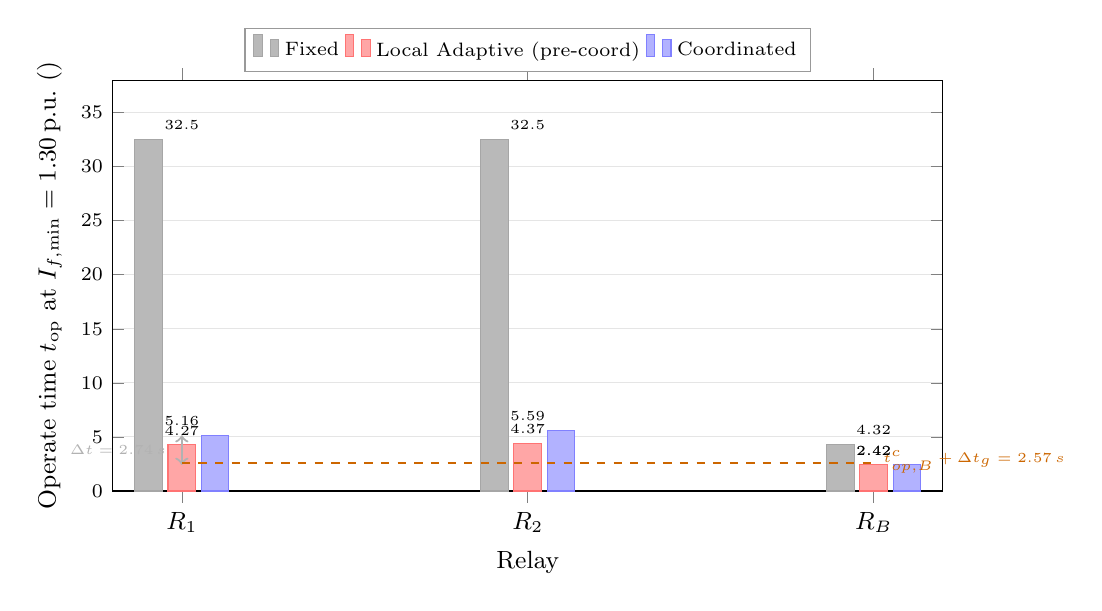
\begin{tikzpicture}
\begin{axis}[
  width=\columnwidth, height=6.8cm,
  ybar=5pt,
  bar width=10pt,
  xlabel={Relay},
  ylabel={Operate time $t_{\mathrm{op}}$ at $I_{f,\min}=1.30\,\mathrm{p.u.}$ (\si{\second})},
  symbolic x coords={$R_1$, $R_2$, $R_B$},
  xtick=data,
  x tick label style={font=\small},
  ymin=0, ymax=38,
  ytick={0,5,10,15,20,25,30,35},
  ymajorgrids=true, grid style={gray!20},
  label style={font=\small},
  tick label style={font=\scriptsize},
  legend style={at={(0.50,1.02)}, anchor=south,
                font=\scriptsize, fill=white, draw=black!40,
                legend columns=3},
  nodes near coords,
  nodes near coords align={vertical},
  every node near coord/.style={font=\tiny},
  clip=false
]

%% Fixed
\addplot[fill=gray!55, draw=gray!70, bar shift=-12pt] coordinates {
  ($R_1$,  32.5)
  ($R_2$,  32.5)
  ($R_B$,   4.32)
};

%% Pre-coord
\addplot[fill=red!35, draw=red!55, bar shift=0pt] coordinates {
  ($R_1$,   4.27)
  ($R_2$,   4.37)
  ($R_B$,   2.42)
};

%% Post-coord
\addplot[fill=blue!30, draw=blue!50, bar shift=12pt] coordinates {
  ($R_1$,   5.16)
  ($R_2$,   5.59)
  ($R_B$,   2.42)
};

%% Grading margin annotation on post-coord R1
\draw[<->, gray!60, thick]
      (axis cs:$R_1$,2.42) -- (axis cs:$R_1$,5.16)
      node[midway, left=2pt, font=\tiny, gray!60] {$\Delta t = 2.74\,\text{s}$};

%% Grading requirement line
\draw[thick, orange!80!black, dashed]
      (axis cs:$R_1$,2.57) -- (axis cs:$R_B$,2.57);
\node[right, font=\tiny, orange!80!black]
      at (axis cs:$R_B$,2.70)
      {$t_{op,B}^c + \Delta t_g = 2.57\,\text{s}$};

\legend{Fixed, Local Adaptive (pre-coord), Coordinated};
\end{axis}
\end{tikzpicture}
